% Scalar instruction entry source: tools/generate_scalar_instruction_catalog.py.
\subsection{\texttt{LH}}
\label{sec:scalar-lh}
\index{LH@\texttt{LH}}
\begin{sloppypar}\noindent\textbf{Purpose.} Loads a signed 16-bit value from memory using register-offset addressing and writes the result to the selected destination.\end{sloppypar}\smallskip
\noindent\textbf{Syntax.}\par
\begin{lstlisting}[style=ptoscalarcode]
lh [SrcL, SrcR<{.sw,.uw,.neg}><<<shamt>], ->RegDst
\end{lstlisting}
\noindent\textbf{Encoding.}\par
\noindent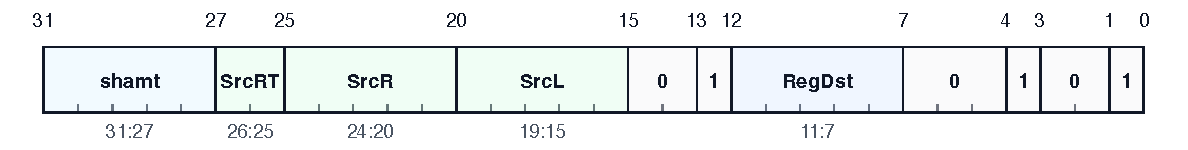
\includegraphics[width=\textwidth]{figs/encoding/scalar_instruction_entries/enc_lh.pdf}\par\smallskip
\begin{description}[leftmargin=0.18\linewidth,style=nextline]
\item[Format] \texttt{L32} \texttt{32-bit} scalar word.
\item[Pattern] \texttt{.................001.....0001001}.
\end{description}
\noindent\textbf{Classification.}\par
\begin{description}[leftmargin=0.18\linewidth,style=nextline]
\item[Category] Load, Store, and Address Generation.
\item[Family] Load Register Offset.
\item[Execution class] \texttt{LDA/BASE\_REG}; uop\_kind=AGU, agu\_kind=LDA, addr\_mode=BASE\_REG.
\end{description}
\noindent\textbf{Operand fields.}\par
\begin{description}[leftmargin=0.18\linewidth,style=nextline]
\item[\texttt{RegDst}] Bits \texttt{11:7 (5b)}. 5-bit scalar destination register that receives the loaded value after any sign or zero extension; X0 discards the load result.
\item[\texttt{SrcL}] Bits \texttt{19:15 (5b)}. 5-bit scalar source register used as the base address for the memory access.
\item[\texttt{SrcR}] Bits \texttt{24:20 (5b)}. 5-bit scalar source register used as the register offset component of the effective address.
\item[\texttt{SrcRType}] Bits \texttt{26:25 (2b)}. 2-bit modifier for SrcR. It selects the encoded source form shown in the syntax, such as signed-word, unsigned-word, negated, or unmodified register input.
\item[\texttt{shamt}] Bits \texttt{31:27 (5b)}. 5-bit shift amount applied to the modified right operand before the ALU or address calculation uses it.
\end{description}
\noindent\textbf{Operation.}\par
\begin{lstlisting}[style=ptoscalarcode]
addr = ComputeAddress(/* per syntax */)
value = Load16(addr)
value = SignExtend(value)
Write(RegDst, value)
\end{lstlisting}
\Needspace{0.08\textheight}
